\subsection*{Case Study}

The case-study used to explore this tools is the modelation made for a project of a subject during our graduation. The subject name was Software Systems Development and it's project was \textit{GCS - Gere Com Saber}, in english, Manages With Knowledge.\\
In the project, GCS is a company which doesn't provide services, but on the other hand, to meet it's clients needs, it has a wide range of suppliers, that GCS subcontracts, who are responsible for the service execution. Multiple suppliers can supply the same service and each  service can be delivered in different ways. Each service can then be composed of multiple activities. As an example, there could be a service called \textit{Shirts til 10Kg} and inside this service there could be activities such as \textit{wash, iron, sewing buttons, etc}.\\
Each activitie of a given service as a stipulated price, and can be hired by a client.\\
The goal of the project was to model and implement a management software, with the same name as the company, that would help the completion of all the tasks inherent to the company.\\

As an example of the UML diagrams used on the test, we will display one image of the general Usecase diagram and an excerpt of the class diagram.

\begin{figure}[H]
\begin{center}
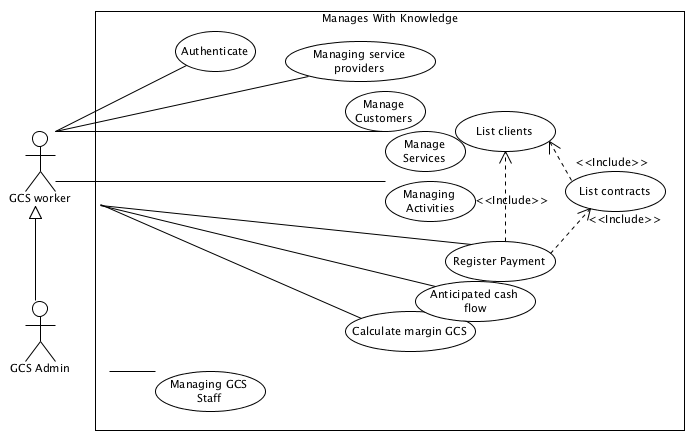
\includegraphics[width=0.9\textwidth]{images/usecase.png}
\caption{The general Usecase of the modelation}\label{img:usecase}
\end{center}
\end{figure} 

\begin{figure}[H]
\begin{center}
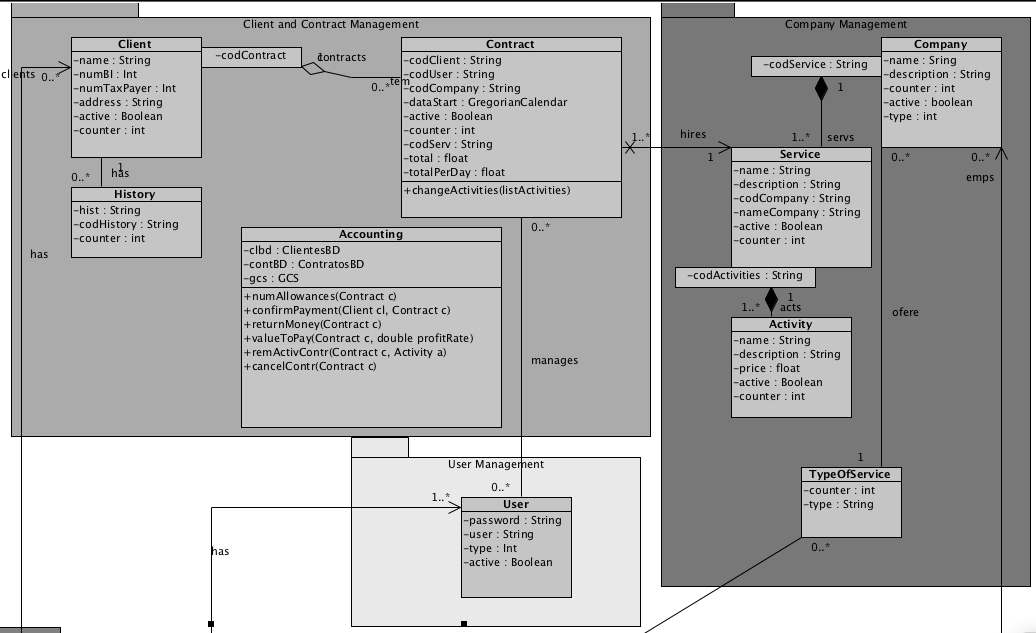
\includegraphics[scale=0.35]{images/classbw.png}
\caption{Excerpt of the Class diagram}\label{img:class}
\end{center}
\end{figure} 
